\iffalse
\let\negmedspace\undefined
\let\negthickspace\undefined
\documentclass[journal,12pt,twocolumn]{IEEEtran}
\usepackage{cite}
\usepackage{amsmath,amssymb,amsfonts,amsthm}
\usepackage{algorithmic}
\usepackage{graphicx}
\usepackage{textcomp}
\usepackage{xcolor}
\usepackage{txfonts}
\usepackage{listings}
\usepackage{enumitem}
\usepackage{mathtools}
\usepackage{gensymb}
\usepackage{comment}
\usepackage[breaklinks=true]{hyperref}
\usepackage{tkz-euclide} 
\usepackage{listings}
\usepackage{gvv}                                        
\def\inputGnumericTable{}                                 
\usepackage[latin1]{inputenc}                                
\usepackage{color}                                            
\usepackage{array}                                            
\usepackage{longtable}                                       
\usepackage{calc}                                             
\usepackage{multirow}                                         
\usepackage{hhline}                                           
\usepackage{ifthen}                                           
\usepackage{lscape}
\usepackage{amsmath}
\usepackage{caption}

\newtheorem{theorem}{Theorem}[section]
\newtheorem{problem}{Problem}
\newtheorem{proposition}{Proposition}[section]
\newtheorem{lemma}{Lemma}[section]
\newtheorem{corollary}[theorem]{Corollary}
\newtheorem{example}{Example}[section]
\newtheorem{definition}[problem]{Definition}
\newcommand{\BEQA}{\begin{eqnarray}}
\newcommand{\EEQA}{\end{eqnarray}}
\newcommand{\define}{\stackrel{\triangle}{=}}
\theoremstyle{remark}
\newtheorem{rem}{Remark}
\begin{document}

\bibliographystyle{IEEEtran}
\vspace{3cm}

\title{GATE: AG-26 2021}
\author{EE23BTECH11038 - Rohith Madhani$^{*}$% <-this % stops a space
}
\maketitle
\newpage
\bigskip
\renewcommand{\thefigure}{\theenumi}
\renewcommand{\thetable}{\theenumi}

\textbf{Question :} Solution of differential equation $y'' + y'+ 0.25y = 0$ with initial values $y(0) = 3$ and $y'(0) = -3.5$ is
\begin{enumerate}
    \item[(A)] $ y = (3-2x)e^{0.5x} $
    \item[(B)] $ y = (3-2x)e^{-0.25x}$
    \item[(C)] $ y = (3-2x)e^{-0.5x}$
    \item[(D)] $ y = (2-3x)e^{-0.5x}$
\end{enumerate} 
\hfill(GATE AG 2021) \\
\solution
\fi

\begin{table}[!h] 
    \centering
    %%%%%%%%%%%%%%%%%%%%%%%%%%%%%%%%%%%%%%%%%%%%%%%%%%%%%%%%%%%%%%%%%%%%%%
%%                                                                  %%
%%  This is the header of a LaTeX2e file exported from Gnumeric.    %%
%%                                                                  %%
%%  This file can be compiled as it stands or included in another   %%
%%  LaTeX document. The table is based on the longtable package so  %%
%%  the longtable options (headers, footers...) can be set in the   %%
%%  preamble section below (see PRAMBLE).                           %%
%%                                                                  %%
%%  To include the file in another, the following two lines must be %%
%%  in the including file:                                          %%
%%        \def\inputGnumericTable{}                                 %%
%%  at the beginning of the file and:                               %%
%%        \input{name-of-this-file.tex}                             %%
%%  where the table is to be placed. Note also that the including   %%
%%  file must use the following packages for the table to be        %%
%%  rendered correctly:                                             %%
%%    \usepackage[latin1]{inputenc}                                 %%
%%    \usepackage{color}                                            %%
%%    \usepackage{array}                                            %%
%%    \usepackage{longtable}                                        %%
%%    \usepackage{calc}                                             %%
%%    \usepackage{multirow}                                         %%
%%    \usepackage{hhline}                                           %%
%%    \usepackage{ifthen}                                           %%
%%  optionally (for landscape tables embedded in another document): %%
%%    \usepackage{lscape}                                           %%
%%                                                                  %%
%%%%%%%%%%%%%%%%%%%%%%%%%%%%%%%%%%%%%%%%%%%%%%%%%%%%%%%%%%%%%%%%%%%%%%



%%  This section checks if we are begin input into another file or  %%
%%  the file will be compiled alone. First use a macro taken from   %%
%%  the TeXbook ex 7.7 (suggestion of Han-Wen Nienhuys).            %%
\def\ifundefined#1{\expandafter\ifx\csname#1\endcsname\relax}


%%  Check for the \def token for inputed files. If it is not        %%
%%  defined, the file will be processed as a standalone and the     %%
%%  preamble will be used.                                          %%
\ifundefined{inputGnumericTable}

%%  We must be able to close or not the document at the end.        %%
	\def\gnumericTableEnd{\end{document}}


%%%%%%%%%%%%%%%%%%%%%%%%%%%%%%%%%%%%%%%%%%%%%%%%%%%%%%%%%%%%%%%%%%%%%%
%%                                                                  %%
%%  This is the PREAMBLE. Change these values to get the right      %%
%%  paper size and other niceties.                                  %%
%%                                                                  %%
%%%%%%%%%%%%%%%%%%%%%%%%%%%%%%%%%%%%%%%%%%%%%%%%%%%%%%%%%%%%%%%%%%%%%%

	\documentclass[12pt%
			  %,landscape%
                    ]{report}
       \usepackage[latin1]{inputenc}
       \usepackage{fullpage}
       \usepackage{color}
       \usepackage{array}
       \usepackage{longtable}
       \usepackage{calc}
       \usepackage{multirow}
       \usepackage{hhline}
       \usepackage{ifthen}

	\begin{document}


%%  End of the preamble for the standalone. The next section is for %%
%%  documents which are included into other LaTeX2e files.          %%
\else

%%  We are not a stand alone document. For a regular table, we will %%
%%  have no preamble and only define the closing to mean nothing.   %%
    \def\gnumericTableEnd{}

%%  If we want landscape mode in an embedded document, comment out  %%
%%  the line above and uncomment the two below. The table will      %%
%%  begin on a new page and run in landscape mode.                  %%
%       \def\gnumericTableEnd{\end{landscape}}
%       \begin{landscape}


%%  End of the else clause for this file being \input.              %%
\fi

%%%%%%%%%%%%%%%%%%%%%%%%%%%%%%%%%%%%%%%%%%%%%%%%%%%%%%%%%%%%%%%%%%%%%%
%%                                                                  %%
%%  The rest is the gnumeric table, except for the closing          %%
%%  statement. Changes below will alter the table's appearance.     %%
%%                                                                  %%
%%%%%%%%%%%%%%%%%%%%%%%%%%%%%%%%%%%%%%%%%%%%%%%%%%%%%%%%%%%%%%%%%%%%%%

\providecommand{\gnumericmathit}[1]{#1} 
%%  Uncomment the next line if you would like your numbers to be in %%
%%  italics if they are italizised in the gnumeric table.           %%
%\renewcommand{\gnumericmathit}[1]{\mathit{#1}}
\providecommand{\gnumericPB}[1]%
{\let\gnumericTemp=\\#1\let\\=\gnumericTemp\hspace{0pt}}
 \ifundefined{gnumericTableWidthDefined}
        \newlength{\gnumericTableWidth}
        \newlength{\gnumericTableWidthComplete}
        \newlength{\gnumericMultiRowLength}
        \global\def\gnumericTableWidthDefined{}
 \fi
%% The following setting protects this code from babel shorthands.  %%
 \ifthenelse{\isundefined{\languageshorthands}}{}{\languageshorthands{english}}
%%  The default table format retains the relative column widths of  %%
%%  gnumeric. They can easily be changed to c, r or l. In that case %%
%%  you may want to comment out the next line and uncomment the one %%
%%  thereafter                                                      %%
\providecommand\gnumbox{\makebox[0pt]}
%%\providecommand\gnumbox[1][]{\makebox}

%% to adjust positions in multirow situations                       %%
\setlength{\bigstrutjot}{\jot}
\setlength{\extrarowheight}{\doublerulesep}

%%  The \setlongtables command keeps column widths the same across  %%
%%  pages. Simply comment out next line for varying column widths.  %%
\setlongtables

\setlength\gnumericTableWidth{%
	44pt+%
	200pt+%
	60pt+%
0pt}
\def\gumericNumCols{3}
\setlength\gnumericTableWidthComplete{\gnumericTableWidth+%
         \tabcolsep*\gumericNumCols*2+\arrayrulewidth*\gumericNumCols}
\ifthenelse{\lengthtest{\gnumericTableWidthComplete > \linewidth}}%
         {\def\gnumericScale{1*\ratio{\linewidth-%
                        \tabcolsep*\gumericNumCols*2-%
                        \arrayrulewidth*\gumericNumCols}%
{\gnumericTableWidth}}}%
{\def\gnumericScale{1}}

%%%%%%%%%%%%%%%%%%%%%%%%%%%%%%%%%%%%%%%%%%%%%%%%%%%%%%%%%%%%%%%%%%%%%%
%%                                                                  %%
%% The following are the widths of the various columns. We are      %%
%% defining them here because then they are easier to change.       %%
%% Depending on the cell formats we may use them more than once.    %%
%%                                                                  %%
%%%%%%%%%%%%%%%%%%%%%%%%%%%%%%%%%%%%%%%%%%%%%%%%%%%%%%%%%%%%%%%%%%%%%%

\ifthenelse{\isundefined{\gnumericColA}}{\newlength{\gnumericColA}}{}\settowidth{\gnumericColA}{\begin{tabular}{@{}p{44pt*\gnumericScale}@{}}t\end{tabular}}
\ifthenelse{\isundefined{\gnumericColB}}{\newlength{\gnumericColB}}{}\settowidth{\gnumericColB}{\begin{tabular}{@{}p{200pt*\gnumericScale}@{}}t\end{tabular}}
\ifthenelse{\isundefined{\gnumericColC}}{\newlength{\gnumericColC}}{}\settowidth{\gnumericColC}{\begin{tabular}{@{}p{60pt*\gnumericScale}@{}}t\end{tabular}}

\begin{tabular}[c]{%
	b{\gnumericColA}%
	b{\gnumericColB}%
	b{\gnumericColC}%
	}

%%%%%%%%%%%%%%%%%%%%%%%%%%%%%%%%%%%%%%%%%%%%%%%%%%%%%%%%%%%%%%%%%%%%%%
%%  The longtable options. (Caption, headers... see Goosens, p.124) %%
%	\caption{The Table Caption.}             \\	%
% \hline	% Across the top of the table.
%%  The rest of these options are table rows which are placed on    %%
%%  the first, last or every page. Use \multicolumn if you want.    %%

%%  Header for the first page.                                      %%
%	\multicolumn{3}{c}{The First Header} \\ \hline 
%	\multicolumn{1}{c}{colTag}	%Column 1
%	&\multicolumn{1}{c}{colTag}	%Column 2
%	&\multicolumn{1}{c}{colTag}	\\ \hline %Last column
%	\endfirsthead

%%  The running header definition.                                  %%
%	\hline
%	\multicolumn{3}{l}{\ldots\small\slshape continued} \\ \hline
%	\multicolumn{1}{c}{colTag}	%Column 1
%	&\multicolumn{1}{c}{colTag}	%Column 2
%	&\multicolumn{1}{c}{colTag}	\\ \hline %Last column
%	\endhead

%%  The running footer definition.                                  %%
%	\hline
%	\multicolumn{3}{r}{\small\slshape continued\ldots} \\
%	\endfoot

%%  The ending footer definition.                                   %%
%	\multicolumn{3}{c}{That's all folks} \\ \hline 
%	\endlastfoot
%%%%%%%%%%%%%%%%%%%%%%%%%%%%%%%%%%%%%%%%%%%%%%%%%%%%%%%%%%%%%%%%%%%%%%

\hhline{|-|-|-|}
	 \multicolumn{1}{|p{\gnumericColA}|}%
	{\gnumericPB{\centering}\gnumbox{Parameter}}
	&\multicolumn{1}{p{\gnumericColB}|}%
	{\gnumericPB{\centering}\gnumbox{Description}}
	&\multicolumn{1}{p{\gnumericColC}|}%
	{\gnumericPB{\centering}\gnumbox{Value}}
\\
\hhline{|-|-|-|}
	 \multicolumn{1}{|p{\gnumericColA}|}%
	{\gnumericPB{\centering}\gnumbox{$y(t)$}}
	&\multicolumn{1}{p{\gnumericColB}|}%
	{\gnumericPB{\centering}\gnumbox{y in time domain}}
	&\multicolumn{1}{p{\gnumericColC}|}%
	{\gnumericPB{\centering}\gnumbox{?}}
\\
\hhline{|-|-|-|}
	 \multicolumn{1}{|p{\gnumericColA}|}%
	{\gnumericPB{\centering}\gnumbox{$y(0)$}}
	&\multicolumn{1}{p{\gnumericColB}|}%
	{\gnumericPB{\centering}\gnumbox{$y$ at $t=0$}}
	&\multicolumn{1}{p{\gnumericColC}|}%
	{\gnumericPB{\centering}\gnumbox{3}}
\\
\hhline{|-|-|-|}
	 \multicolumn{1}{|p{\gnumericColA}|}%
	{\gnumericPB{\centering}\gnumbox{$y'(0)$}}
	&\multicolumn{1}{p{\gnumericColB}|}%
	{\gnumericPB{\centering}\gnumbox{$y'$ at $t=0$}}
	&\multicolumn{1}{p{\gnumericColC}|}%
	{\gnumericPB{\centering}\gnumbox{-3.5}}
\\
\hhline{|-|-|-|}
\end{tabular}

\ifthenelse{\isundefined{\languageshorthands}}{}{\languageshorthands{\languagename}}
\gnumericTableEnd
    \caption{Given parameters}
    \label{table:gate21ag26}
\end{table}
By applying laplace transform to the differential equation,
\begin{align}
    y''+y'+0.25y &\Large\xleftrightarrow{\mathcal{L}} s^2Y(s)-sy(0)-y'(0)+sY(s)-y(0)+0.25Y(s)
\end{align}

\begin{align}
    Y(s)(s^2 + s + 0.25) &= 3s - 0.5 \\
    \implies Y(s) &= \frac{3s-0.5}{s^2 + s + 0.25} \\
    &= \frac{3}{s+0.5} - \frac{2}{(s+0.5)^2};Re(s) > -0.5 \label{parfrac}
\end{align}

As we know,
\begin{align}
    \frac{b}{(s+a)^n} &\Large\xleftrightarrow{\mathcal{L}^{-1}}\frac{b}{(n-1)!} t^{n-1} e^{-at} u(t)
\end{align}

By taking inverse laplace of \eqref{parfrac}, we get
\begin{align}
    y(t) &= \frac{3}{0!}e^{-0.5t}u(t)-\frac{2}{1!}te^{-0.5t}u(t) \\
    \implies y(t) &= \sbrak{(3-2x)e^{-0.5t}}u(t)
\end{align}
Hence the correct answer is option (C)
\newpage

\begin{figure}[t]
    \centering
    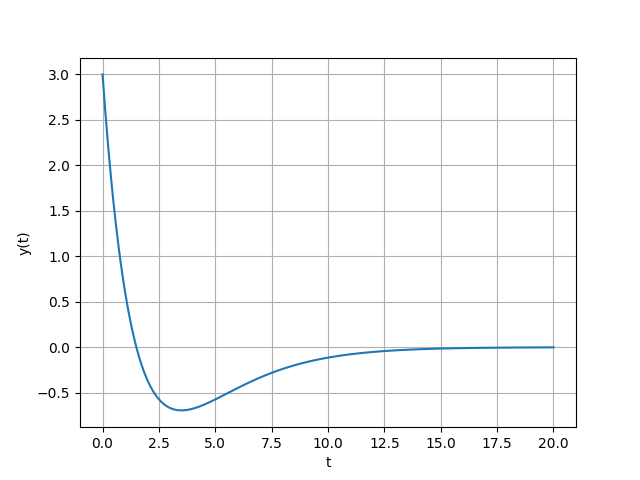
\includegraphics[width=\columnwidth]{2021/AG/26/figs/fig1.png}
    \caption{$y(t) = \sbrak{(3-2t)e^{-0.5t}}u(t)$}
    \label{fig:gate21ag26}
\end{figure}

%\end{document}
